\documentclass{article}
\title{CUDA Parallel Programming\\Homework 1}
\usepackage{graphicx}
\usepackage[UTF8]{ctex}
\CTEXoptions[today=old]
\author{40647007S 朱健愷}

\begin{document}
	\maketitle
	\section{Source codes}
	\subsection{File Layout}
	\begin{itemize}
		\item matAdd.cu - Main code containing both CPU and GPU code
		\item Makefile - Script to auto generate executable from code
		\item experiment.sh - Script to auto generate results of matrix addition using different block size
		\item Output\textunderscore* - Output result of matrix addition using different block size, the suffix represent the block size per dimension in 2D
		\item notebook/*.png - Plots concluding output result
	\end{itemize}
	
	
	\subsection{Usage}
	Run the experiment.sh script
	
	\begin{verbatim}
	sh experiment.sh
	\end{verbatim}
	
	And it will produce matrix addition statistical result using different block size.
	\section{Result}
	\subsection{Experiment environment}
	I ran my code on workstation provided in course, below is the Setup of workstation
	\begin{itemize}
		\item Operating system: Linux version 4.19.172 (root@twcp1)\\(gcc version 6.3.0 20170516 (Debian 6.3.0-18+deb9u1))
		\item CPU: Intel(R) Core(TM) i7-4790 CPU @ 3.60GHz
		\item GPU: Nvidia GTX 1060 6GB
		\item Memory: 32GB 
	\end{itemize}
	\subsection{Input time}
	The input time is the time elapsed when copying data from main memory to GPU memory.
	
	After running the code in different block size, I observed that input time around 52(ms), which is irrelevant to block size.
	
	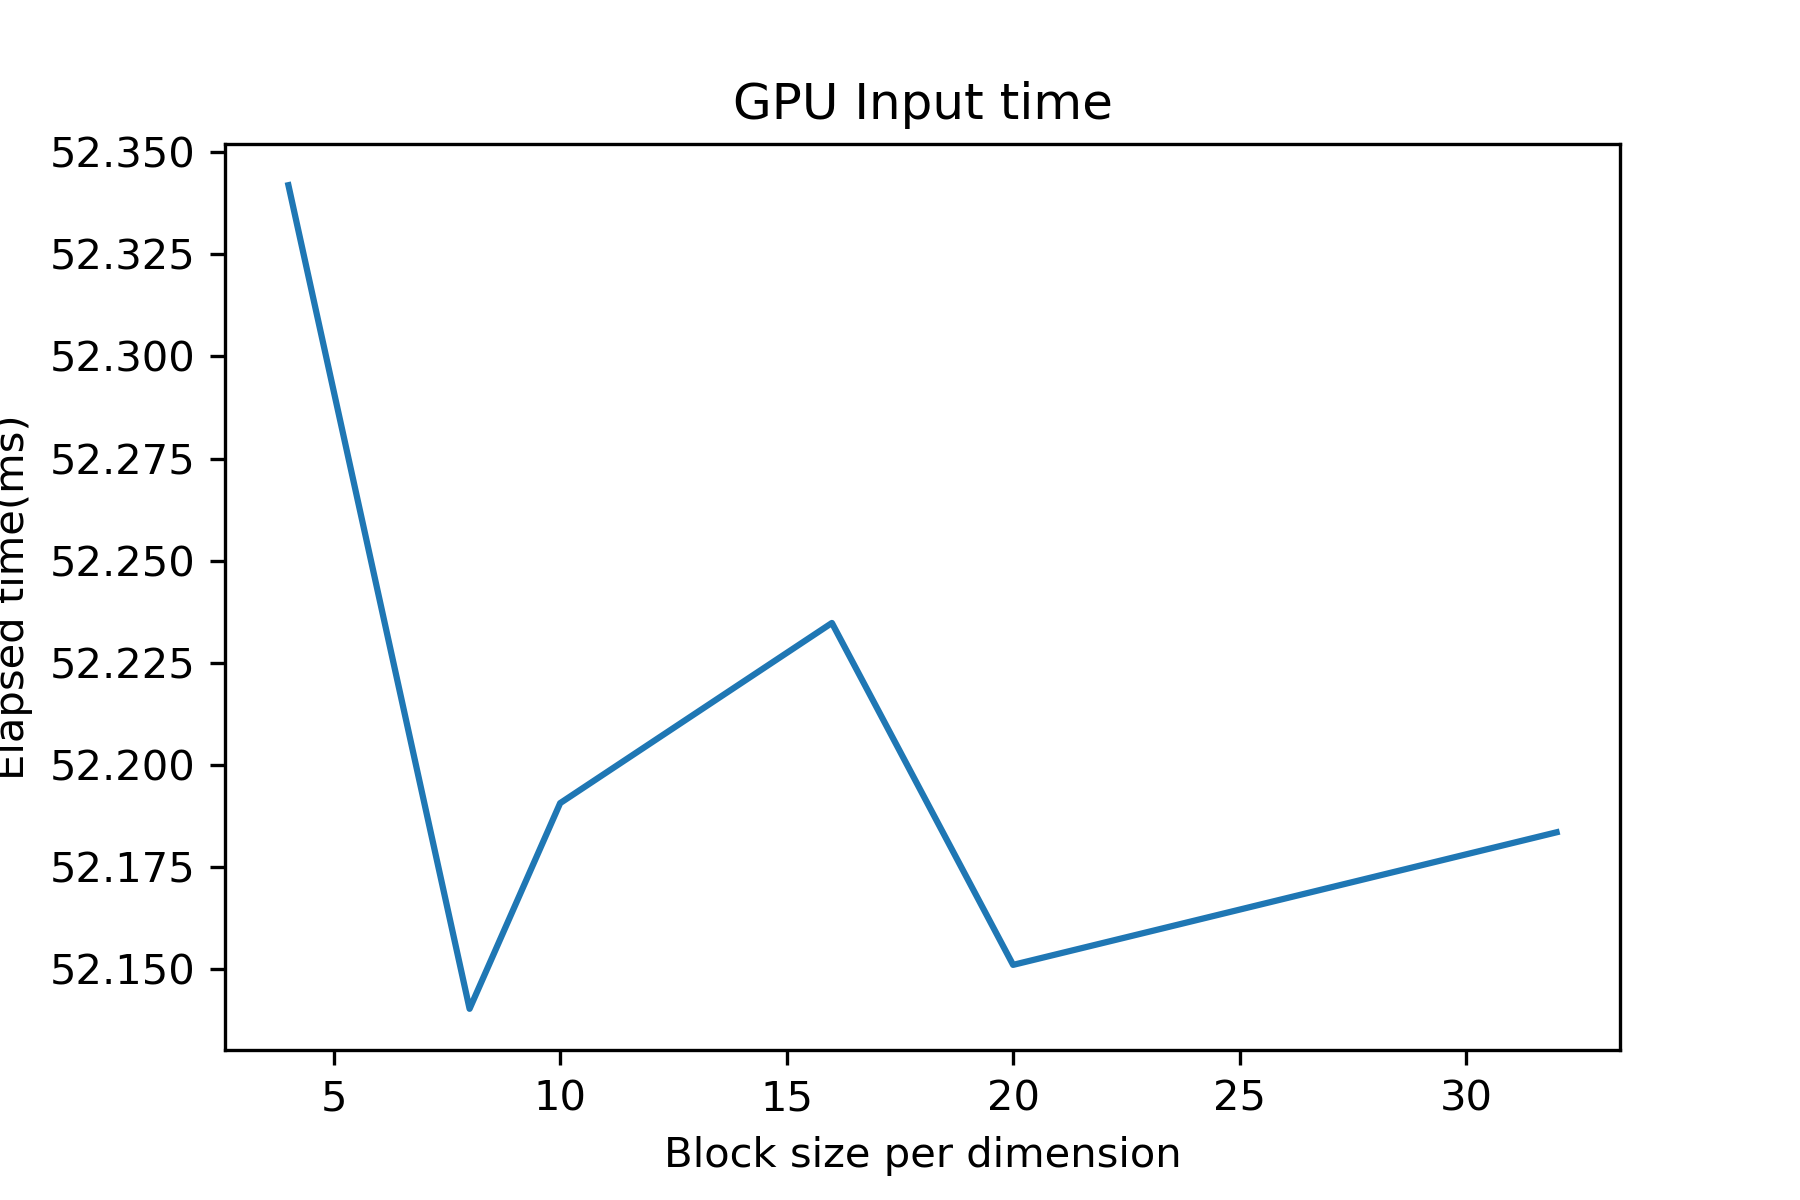
\includegraphics[width=\linewidth]{notebook/gpu_input_time}
	
	It is probably because of the input depends only on memory access, it didn't involved in the matrix addition "operation", so it didn't be affected by block size.	
	\subsection{Processing time}
	The process time is the time elapsed when doing matrix addition operation
	
	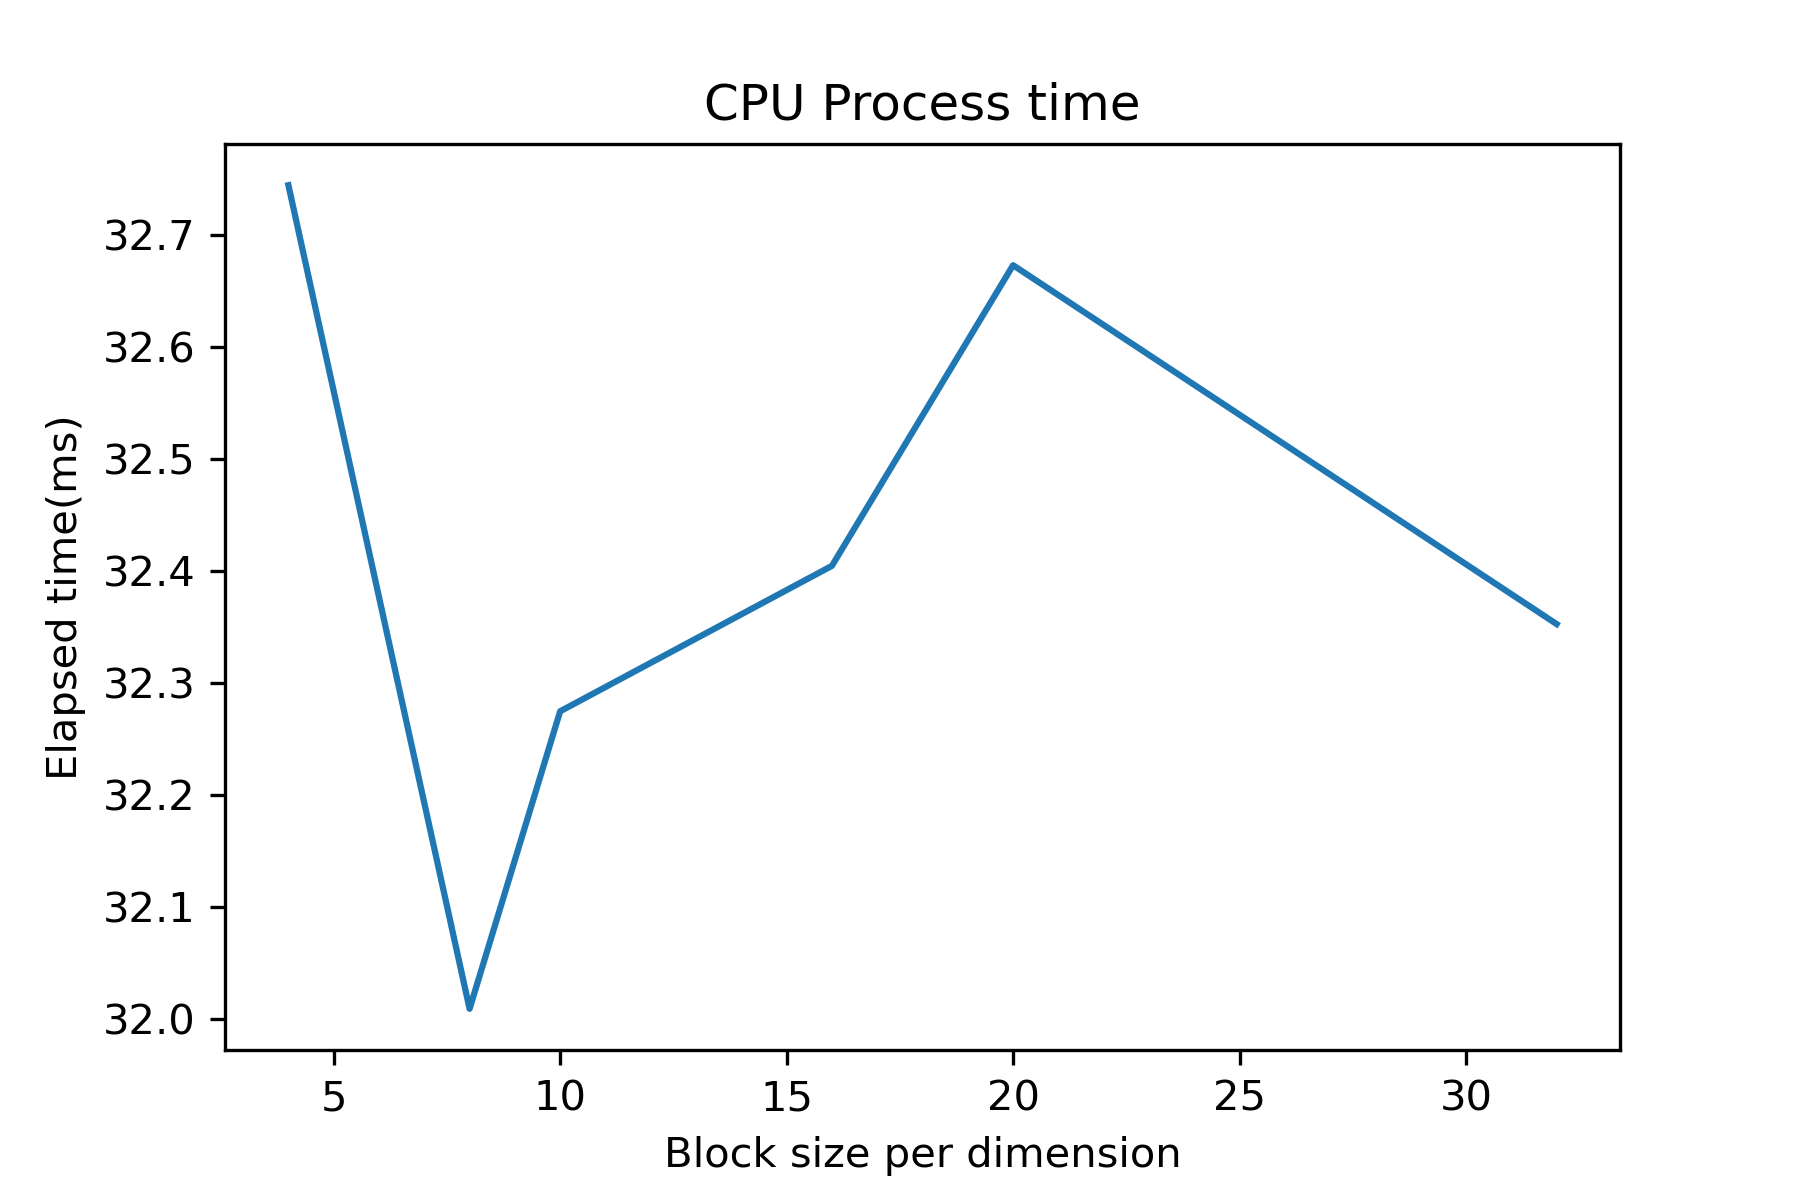
\includegraphics[width=\linewidth]{notebook/cpu_process_time}
	
	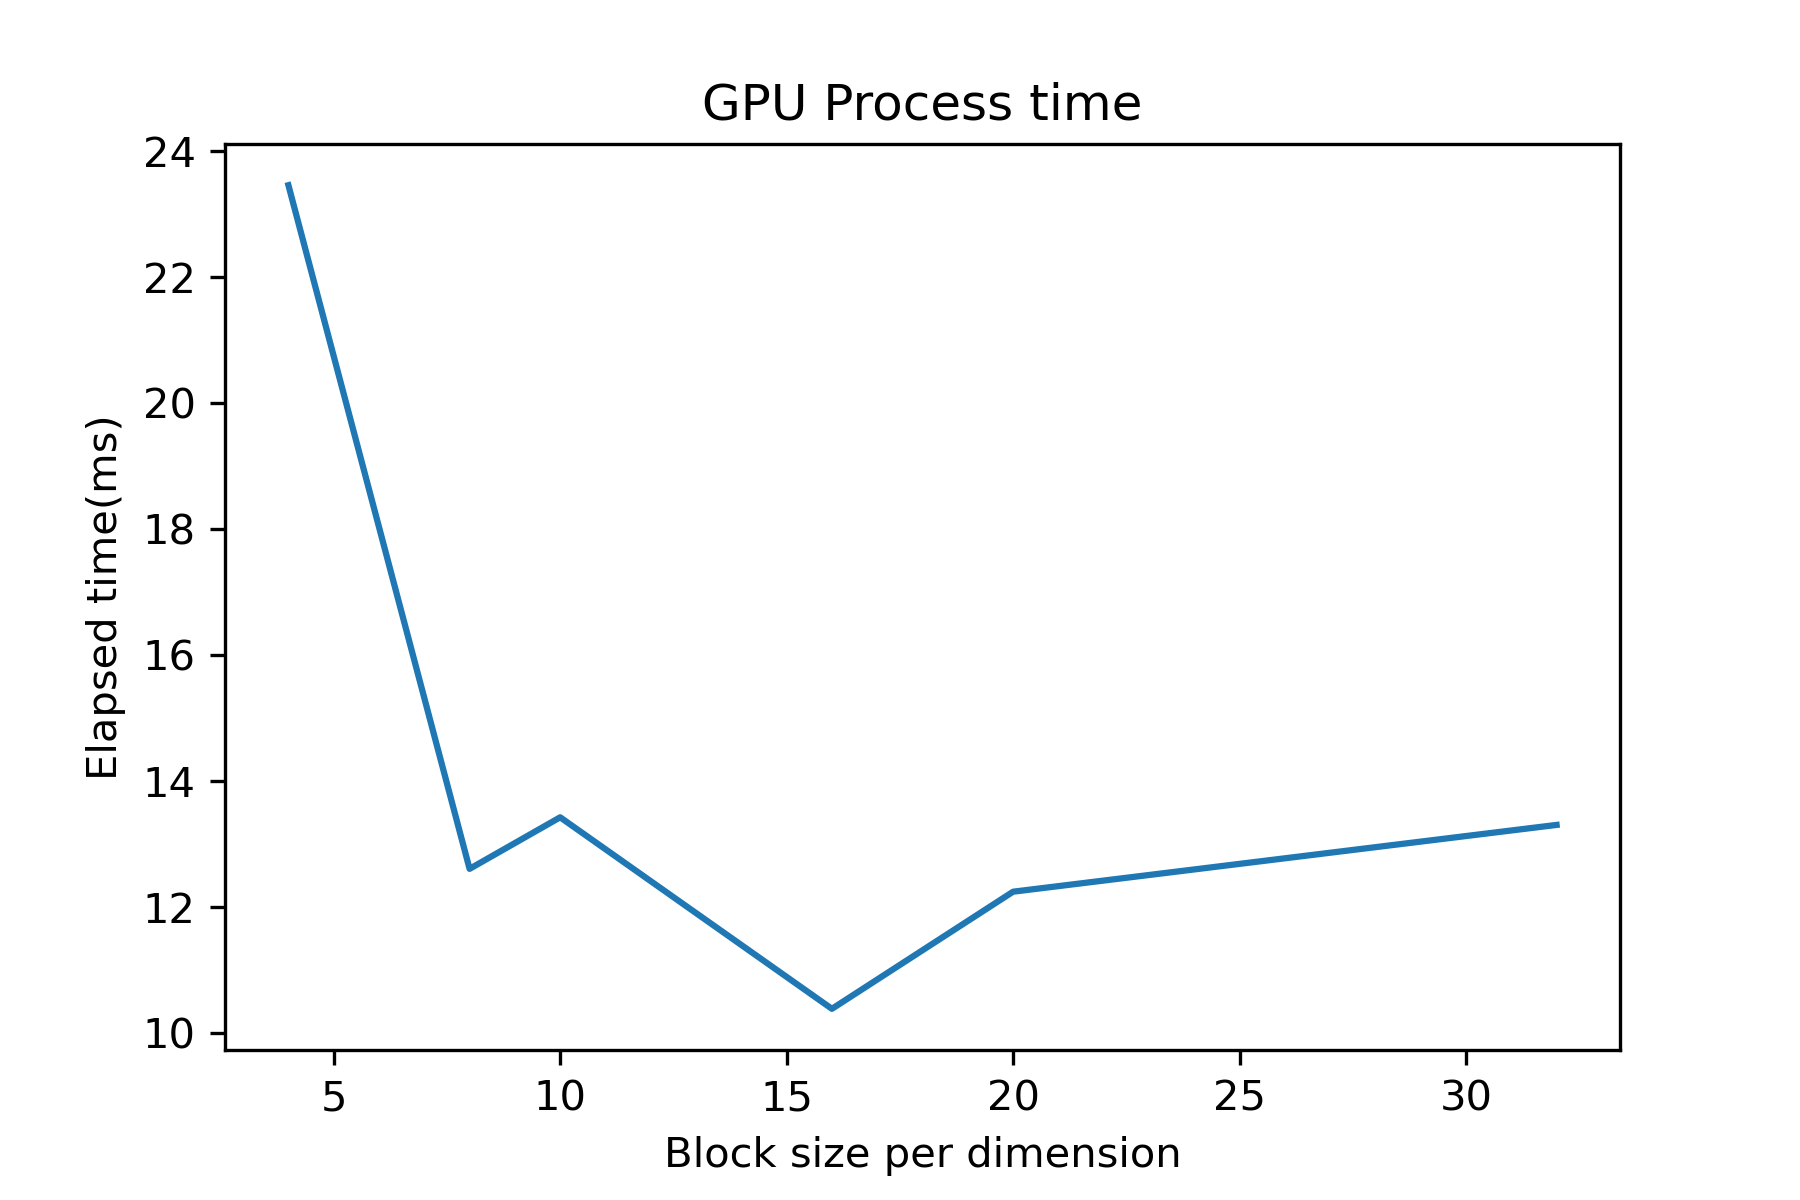
\includegraphics[width=\linewidth]{notebook/gpu_process_time}
	
	I observed that the processing time is much faster than input time in all 6 block size setup.
	But after having a comparison of processing time between different block size, I observed that in matrix addition, (4, 4) block size have one time bigger processing time to any other block size approximately, and the processing time didn't decrease further after reaching some block size setup.
	
	That's because that when we are doing operation, we have to order blocks and threads to work, so the operations apparently have association with block size setup.
	
	In comparison with CPU Processing time, we can observe that the GPU processing time is better than CPU processing time in 6 block size setup, it’s because that the matrix addition doesn’t have data dependency while doing addition with each other, so each cell of GPU can do it simultaneously. We just have to dispatch threads to do their own work once, and the operation is done, while CPU have to do the addition operation sequentially, which means it should deal with every cell of matrix to add them together. 
	
	\subsection{Output time}
	The output time is the time elapsed when copying data from GPU memory to main memory.
	
	After running the code in different block size, I observed that output time around 45(ms), which seems irrelevant to block size. The reason why it's irrelevant to block size is similar to the input time one.
	
	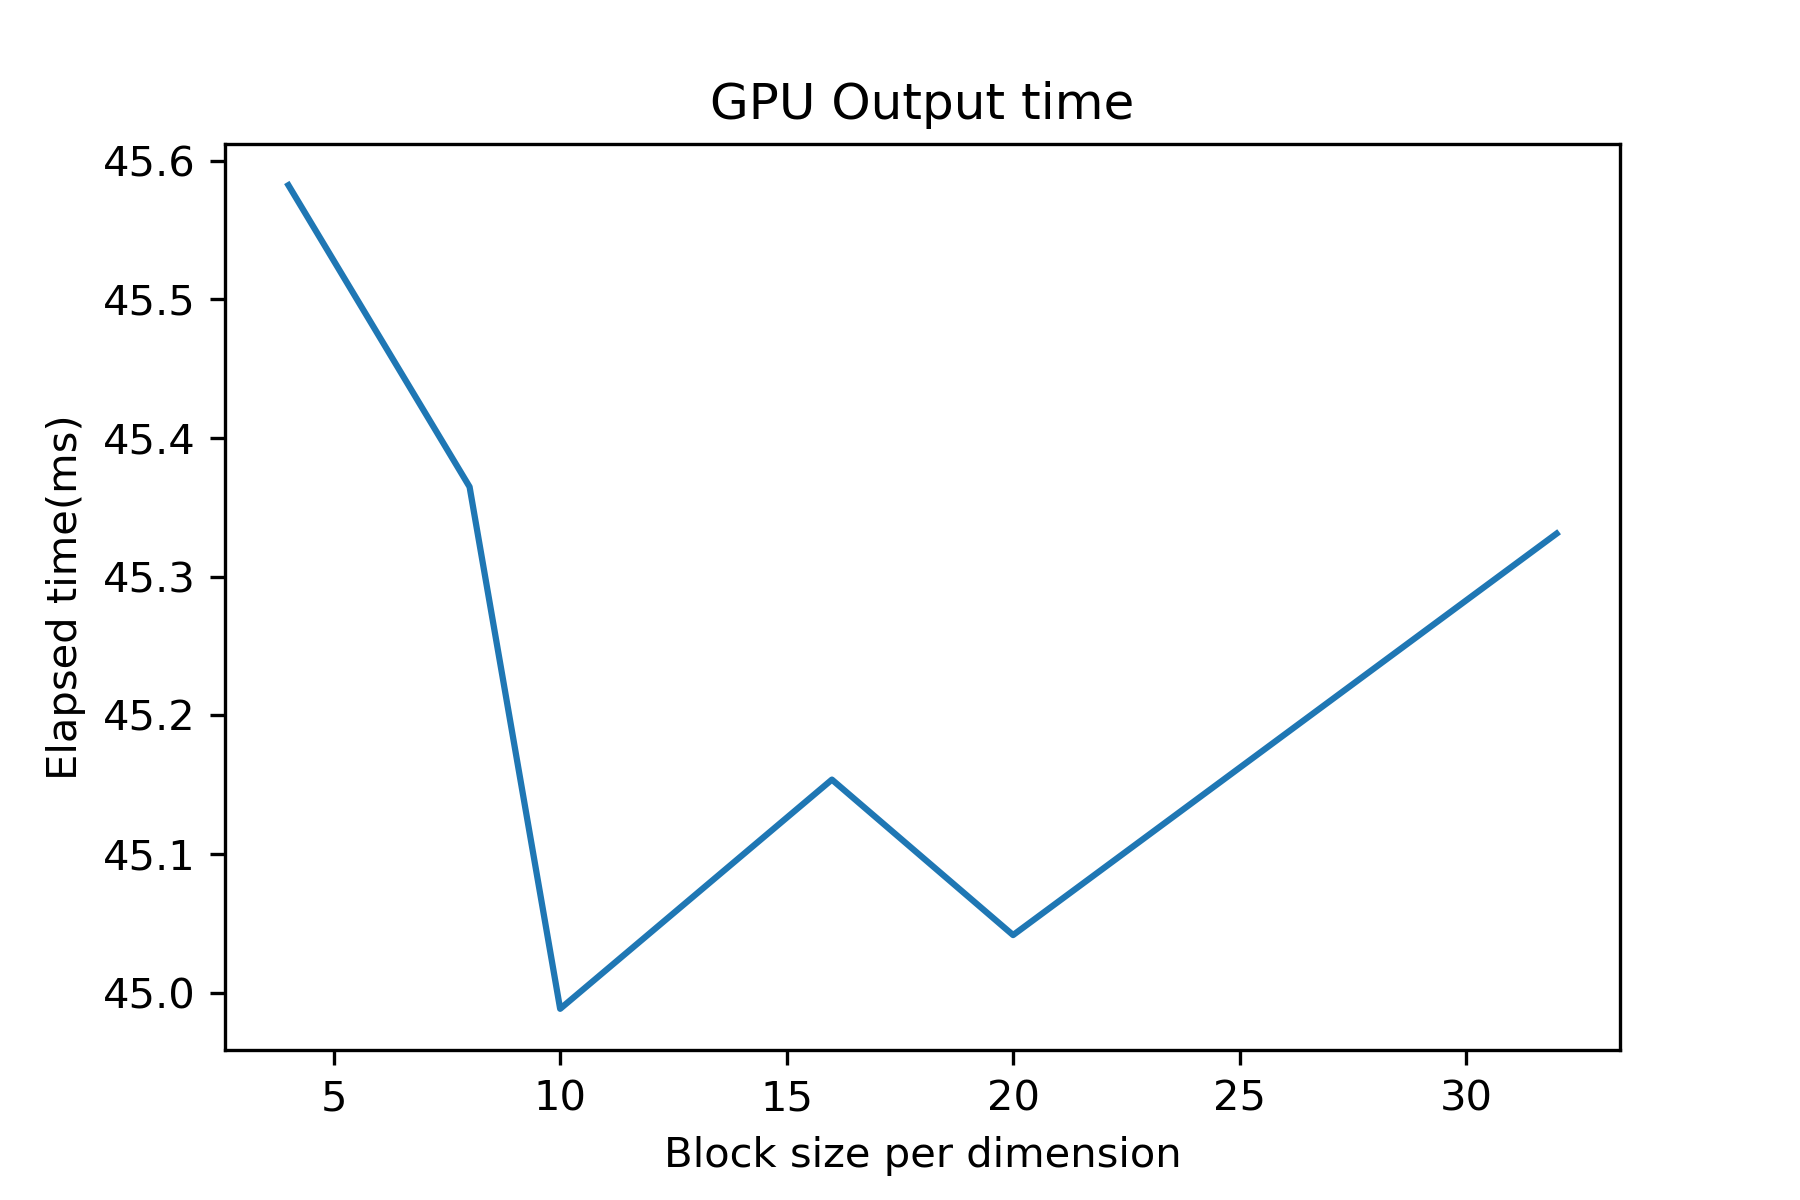
\includegraphics[width=\linewidth]{notebook/gpu_output_time}
	\subsection{Total time}
	The total time is the time elapsed when doing above three work, the GPU have input, processing, output time, while the CPU only have processing time.
	
	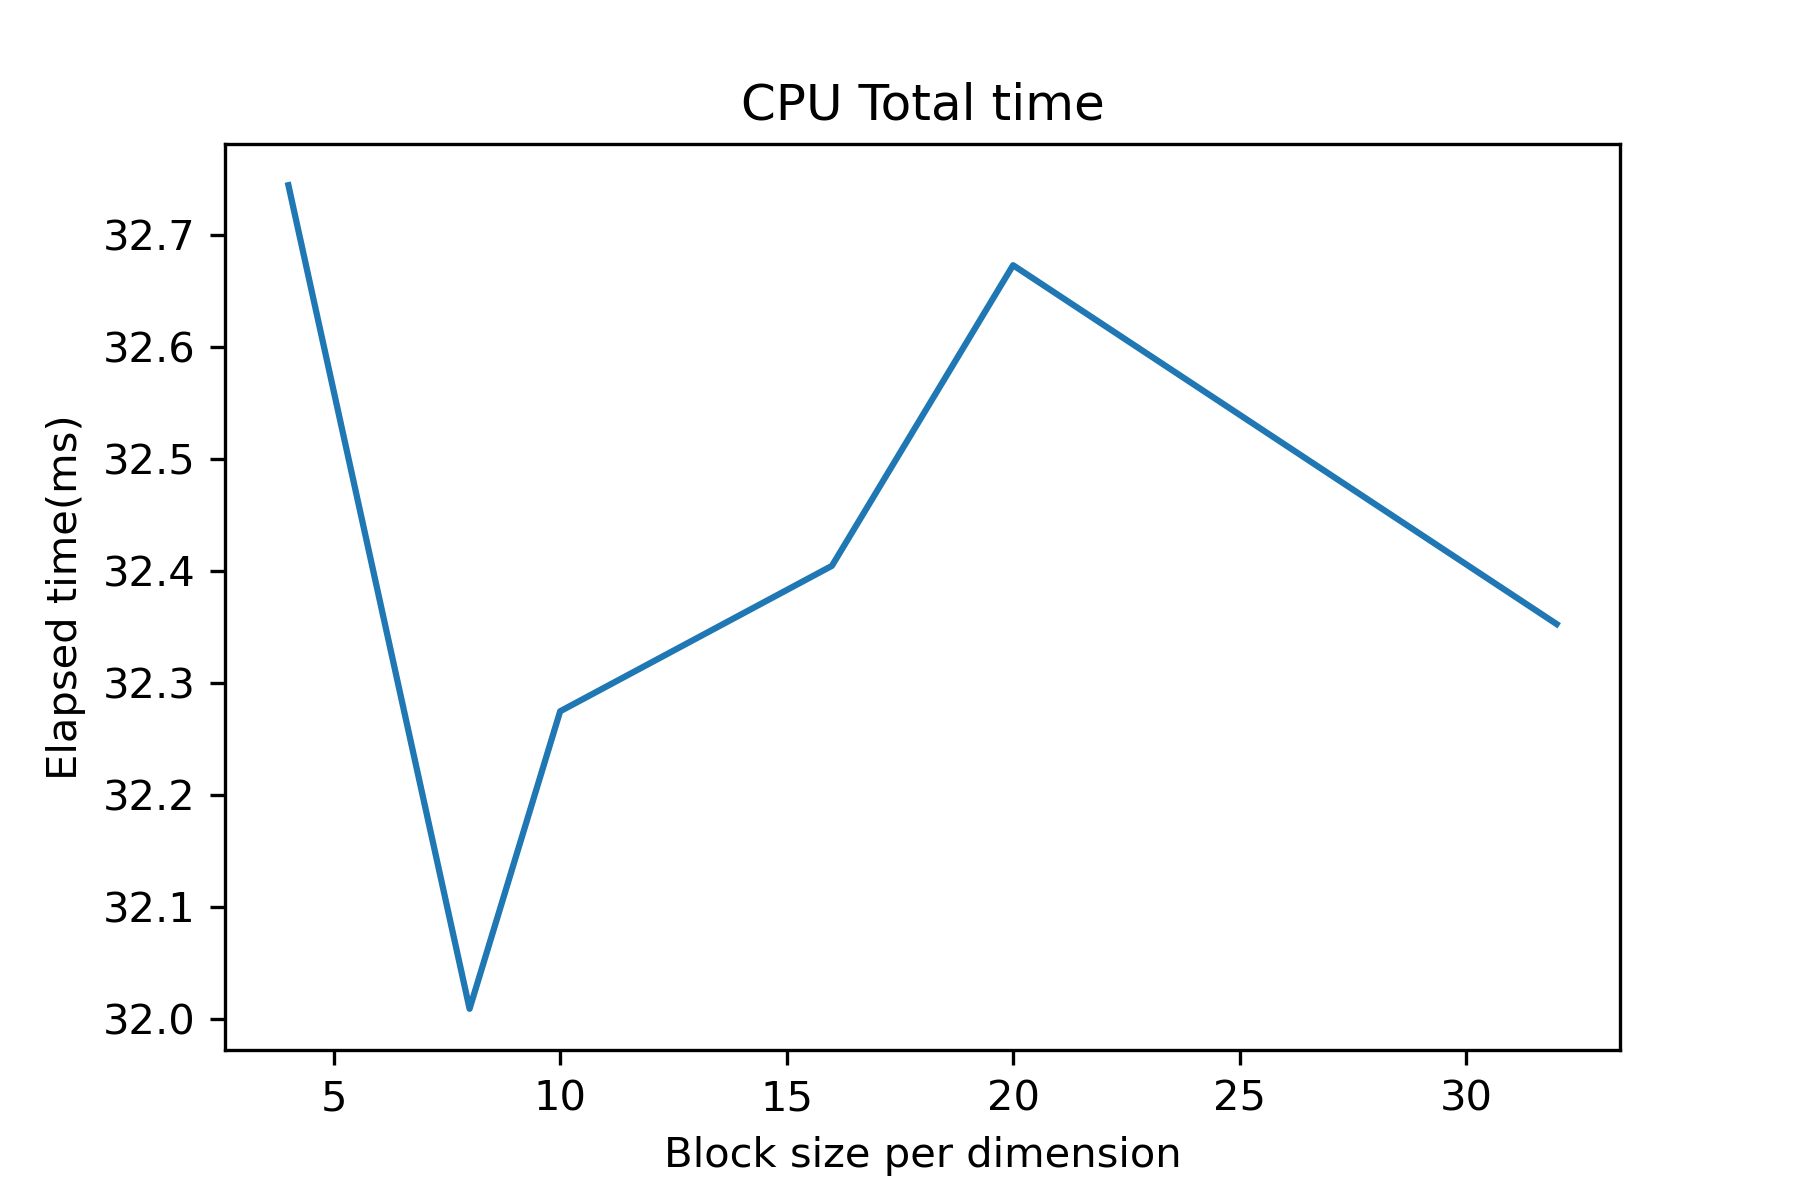
\includegraphics[width=\linewidth]{notebook/cpu_total_time}
	
	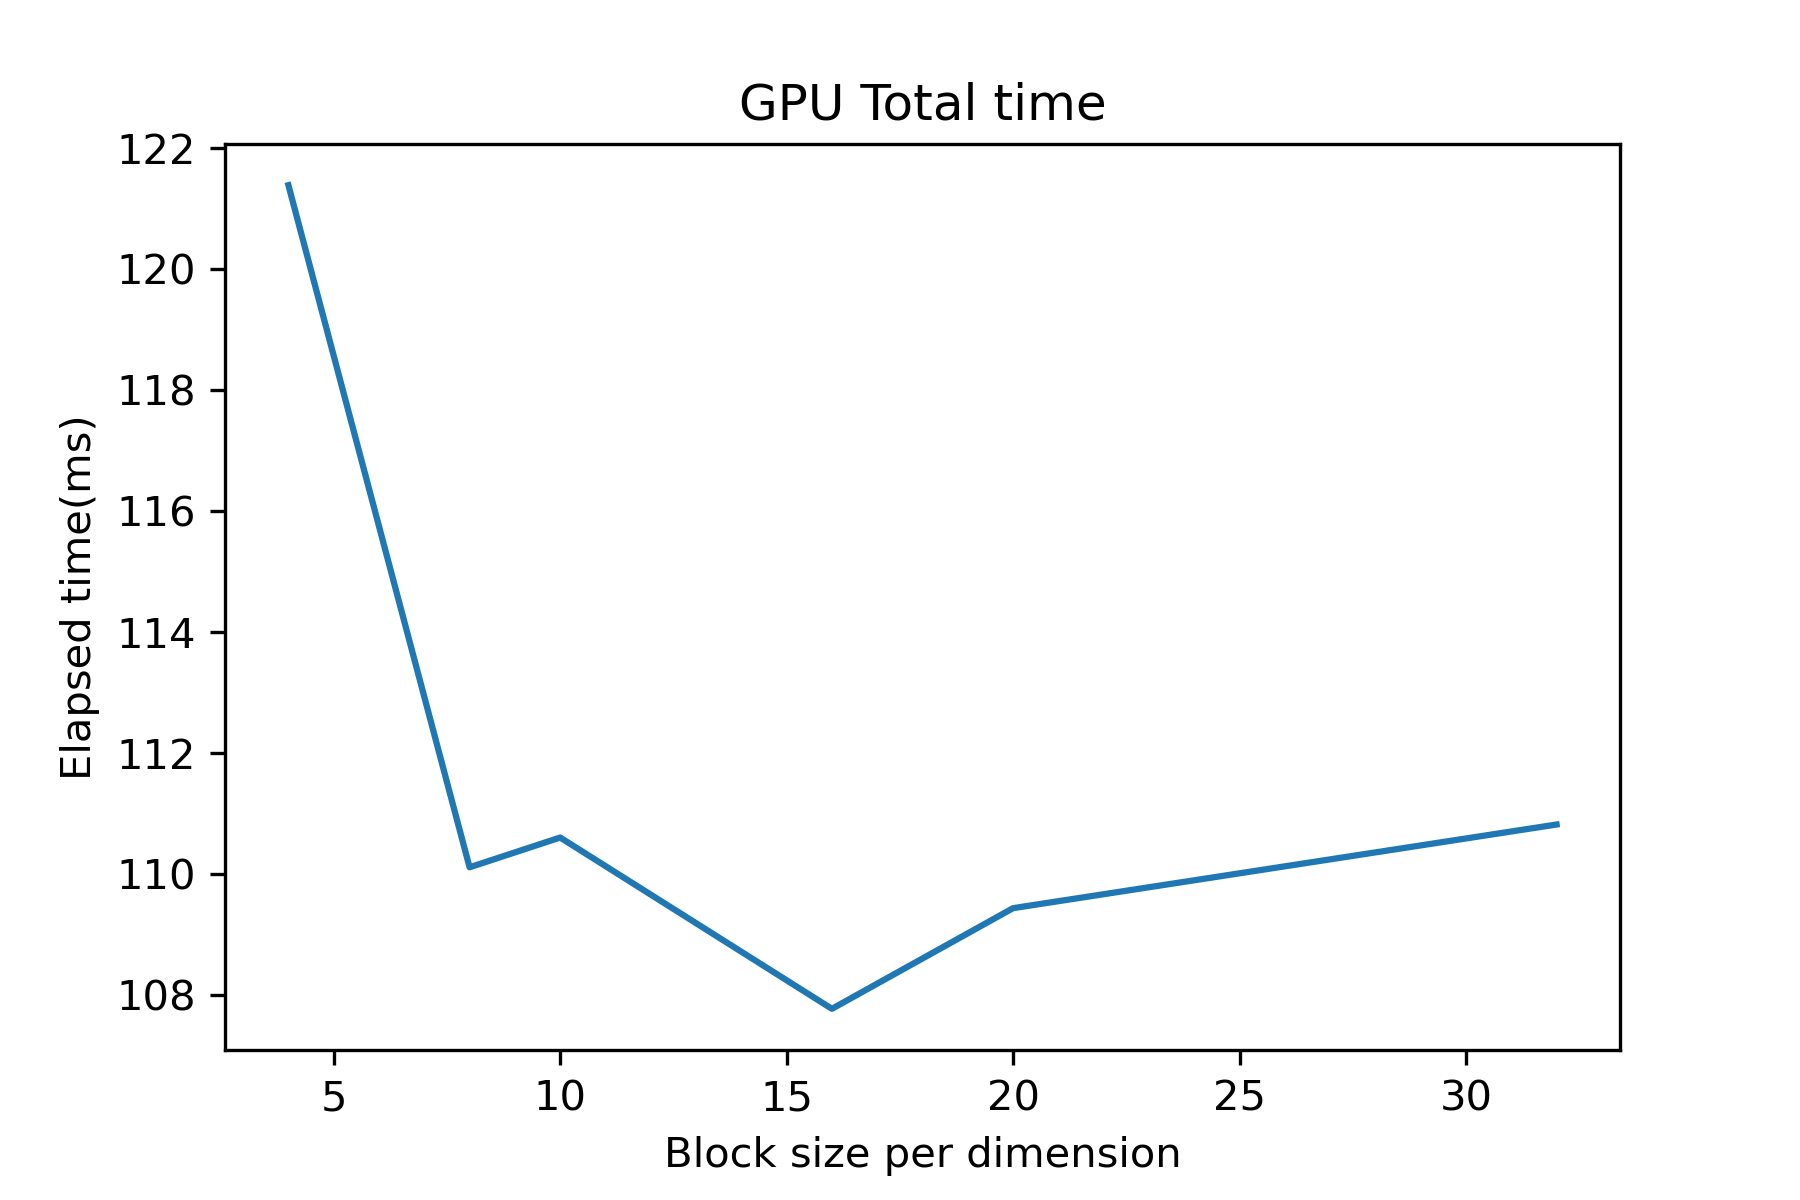
\includegraphics[width=\linewidth]{notebook/gpu_total_time}
	
	We can observe that although GPU has pretty decent processing time than CPU does, after adding consideration of I/O time, its total time looks not good.
	
	\section{Discussion}
	From this assignment we can observe that
	\begin{itemize}
		\item GPU is more suitable in doing operations which don’t have much data dependency between cells than CPU
		\item Adjusting block size do help improving computation time
		\item After reaching some block size setup, the computation time won’t decrease further
		\item I/O time is an unignorable issue in designing a CUDA parallel computation program
	\end{itemize}
\end{document}